\chapter{Regroupement Modulaire et description des flux de données}

Dans la \autoref{fig:25-regroupement_modulaire}, nous pouvons identifier les multiples parties composant notre application.

\begin{figure}[h]
    \centering
    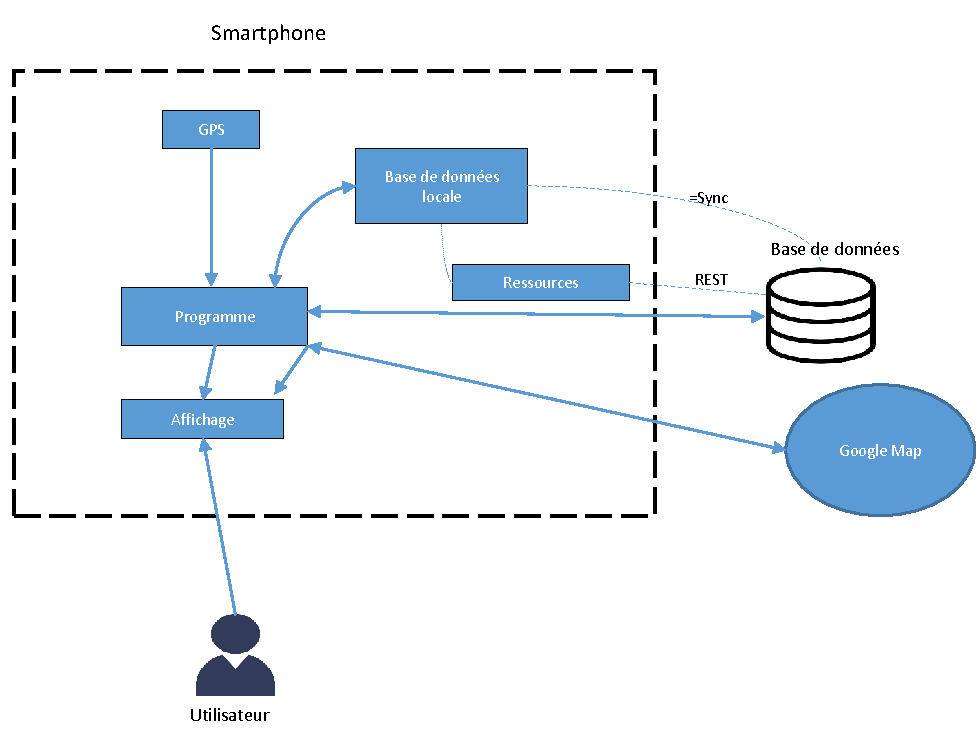
\includegraphics[keepaspectratio, width=2\textwidth/2, height=2\textheight/5]{ima/regroupement_modulaire}
    \caption{Schéma fonctionnel de notre projet.}
    \label{fig:25-regroupement_modulaire}
\end{figure}

\section{GPS}
GhostRun a besoin de récupérer le trajet de l'utilisateur, et pour pouvoir connaitre l'évolution de la position de l'utilisateur
dans le but de l'afficher lors d'un futur trajet. De ce fait l'intervalle de temps entre 2 relevé de position doit être faible.
(de l'ordre de la seconde.)
Le fait de connaitre la position de l'utilisateur à cette fréquence nos permet d'afficher un fantôme qui se déplace de manière continue dans le temps,
mais aussi de connaitre l'évolution de la vitesse au fûr ét à mesure du trajet.
% Expliquer ce que c'est, ce pourquoi l'appli s'en sert et à quelle fréquence, etc..

\section{Base de données}
Nous allons utiliser deux bases de données une locale et une autre à distance. Nous allons stocker différentes informations comme les données et statistiques des différents trajets, les positions favorites des utilisateurs, ces identifiants de connexions et leurs historiques de connexions.
Le programme principal communiquera avec la base de données locale et cette base de données se synchronisera avec la base de données distante. Des ressources devront passer par une api REST avant d’être stockées sur le serveur distant.



\section{Google Maps}
Nous allons utilisé l'API de Google Maps pour avoir la carte sur notre application.
Elle permettra à l'utilisateur de voir sa position actuelle et de préparer une course en choisissant une position de départ et une position d'arrivée.
L'utilisateur pourra de plus enregistrer des positions prédéfinies sur cette carte pour ne pas avoir à réécrire des adresses.

\section{Ressources externes}
Les ressources externes permettent de stocker tout ce qui ne peut pas être stocké dans la base de données.
Par exemple, si l'utilisateur souhaite ajouter une image pour décrire son trajet, celle-ci ira dans les ressources externes et à l'aide de l'api REST,
les ressources seront transférés à la base de données externe.

\section{Affichage}
L'interface Homme-Machine permettra à l'utilisateur de voir la carte de Google Maps pour voir sa position actuelle, le trajet en cours,
ainsi que son fantôme en temps réel pour savoir si il arrive à aller plus vite que lui.
Il pourra choisir facilement le trajet de son choix, son moyen de transport et voir ses statistiques sur celui-ci (comme sa vitesse moyenne, maximale).
Tout les trajets enregistrés par l'utilisateur seront consultables à tout moment dans un tableau pour que l'utilisateur voit toutes ses statistiques en appuyant simplement sur un bouton.